\documentclass[addpoints]{exam}
\usepackage[utf8]{inputenc}
\usepackage[portuguese]{babel}
\usepackage[LGRgreek]{mathastext}
\usepackage{graphicx,graphics}
\usepackage{hyperref}
%\usepackage{framed}
\usepackage{multirow}
\usepackage{booktabs}
\usepackage{pdfpages} 

\footer{}{\thepage}{}

%%% INÍCIO DOS COMANDOS ACRESCENTADOS NO NETBOOK %%%%%%%%%%%%%%%%%%%
\newcommand*{\renameenviron}[1]{%
  \expandafter\let\csname exam-#1\expandafter\endcsname
      \csname #1\endcsname
  \expandafter\let\csname endexam-#1\expandafter\endcsname
      \csname end#1\endcsname
  \expandafter\let\csname #1\endcsname\relax
  \expandafter\let\csname end#1\endcsname\relax
}
\renameenviron{framed}
\renameenviron{shaded}
\renameenviron{leftbar}
%%% FIM DOS COMANDOS ACRESCENTADOS NO NETBOOK %%%%%%%%%%%%%%%%%%%
\usepackage{framed}

\renewcommand{\arraystretch}{1.3}
%\setlength{\tabcolsep}{pt}
 
\pointpoints{ponto}{pontos}
\bonuspointpoints{ponto extra}{pontos extra}
 
\totalformat{Pregunta \thequestion: \totalpoints pontos}
 
\chqword{Pregunta}
\chpgword{Página}
\chpword{Pontos}
\chbpword{Pontos extra}
\chsword{Pontos obtidos}
\chtword{Total}

\hqword{Questão}
\hpgword{Página}
\hpword{Pontos}
\hsword{Pontos obtidos}
\htword{Total}

 
\begin{document}
 
\large

\begin{center}
\Large
\textbf{Laboratório de Eletrônica Básica II – EE641}
\end{center}

\large
\vspace{2mm}

\noindent\textbf{Profs.:} Dr. Eduardo T. Costa\hfill \textbf{Turma 01/2022} \\
\textbf{PED:} Mathias Scroccaro Costa \hfill %\textbf{e-mail:} mathias.scroccaro@gmail.com

\normalsize
 
\vspace{5mm}
 

 
\noindent\makebox[0.72\textwidth]{Nome: \enspace\hrulefill}
\hfill
\makebox[0.2\textwidth]{RA: \enspace\hrulefill}

\vspace{5mm}

\noindent\makebox[0.72\textwidth]{Nome: \enspace\hrulefill}
\hfill
\makebox[0.2\textwidth]{RA: \enspace\hrulefill}

\vspace{5mm}

\noindent\makebox[0.72\textwidth]{Nome: \enspace\hrulefill}
\hfill
\makebox[0.2\textwidth]{RA: \enspace\hrulefill}



%\begin{center}
%\gradetable[h][questions]
%\end{center}

\vspace{2mm}


\begin{center}
\large
\textbf{AJUSTE DE \textit{OFFSET} E INSERÇÃO DE RUÍDO}
\normalsize
\end{center}

\begin{questions}

\section*{Atenuador e somador}

\question \label{part:circuito} Complete o circuito Conversor Digital para Analógico acrescentando o circuito atenuador somador, à direita do nó ``Teste DAC'', conforme mostra o esquemático da Figura \ref{cir:1}. Continue soldando os componentes na \textbf{placa furada padrão}.

\begin{figure}[h!]
\begin{center}
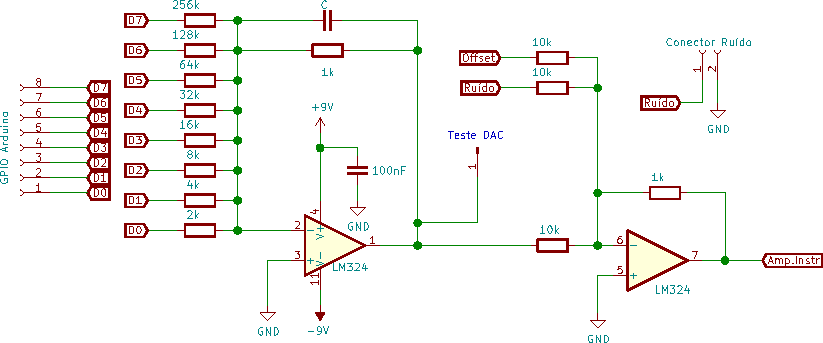
\includegraphics[width=\textwidth]{imagens/1.pdf}
\end{center}
\caption{Circuito completo gerador de sinais.}
\label{cir:1}
\end{figure}

\pagebreak

\begin{parts} 

\part \label{part:1} Utilizando um gerador de sinais, insira uma forma de onda senoidal com 1 V de amplitude e frequência de 10 Hz sobre o nó ``D0''. Com auxílio de um osciloscópio, monitore através do canal 1 o gerador de sinais; e com o canal 2 a forma de onda observada em ``Amp.Instr''. Utilizando o recurso ``Measure'', mostre no display a tensão de pico a pico de ambos os canais. Salve os sinais vistos no osciloscópio em uma única figura, imprima-a e anexe-a ao relatório. A amplitude da forma de onda observada é coerente com o esperado?

\pagebreak

\part Ainda com o \textit{setup} montado do item (\ref{part:1}), verifique na prática a frequência de corte do filtro no primeiro estágio somador:
\begin{subparts}
\subpart \label{subpart:1} Para frequência inicial de 10 Hz, anote a tensão de pico a pico vista em ``Amp.Instr'';
\subpart Gradualmente, aumente a frequência do gerador de sinais até o momento em que a tensão de pico a pico vista em ``Amp.Instr'' é -3 dB do valor do item (\ref{subpart:1}).
\subpart Salve a forma de onda de entrada (D0) e saída (Amp.Instr) em que ocorre a frequência de corte em uma única figura, imprima-a e anexe-a ao relatório.
\subpart A frequência de corte observada na prática é coerente com a esperada? Comente eventuais discrepâncias. 
\end{subparts} 

\pagebreak

\part Utilizando um gerador de sinais, insira uma forma de onda senoidal com 1 V de amplitude e frequência de 300 Hz sobre o nó ``Conector Ruído''. Com auxílio de um osciloscópio, monitore através do canal 1 o gerador de sinais; e com o canal 2 a forma de onda observada em ``Amp.Instr''. Salve os sinais vistos no osciloscópio em uma única figura, imprima-a e anexe-a ao relatório.

\end{parts}

\pagebreak

\section*{Circuito de ajuste de \textit{offset}}

\question Monte o circuito de ajuste de \textit{offset} em \textbf{placa furada padrão}, conforme mostra o esquemático da Figura \ref{cir:2}. Utilize Cin = 1 uF. \textbf{Atenção:} a tensão do nó ``offset'' deve ser conectada ao nó correspondente no circuito do item (\ref{part:circuito}).

\begin{figure}[h!]
\begin{center}
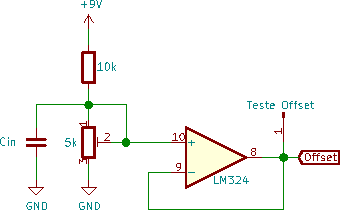
\includegraphics[width=0.6\textwidth]{imagens/2.pdf}
\end{center} 
\caption{Circuito atenuador e filtro.}
\label{cir:2}
\end{figure}

\begin{parts}
\part Qual é faixa de tensões possíveis ao nó ``Offset''? Utilize o trimpot para verificar os valores e meça com multímetro.
\begin{framed}
Tensão mínima = \hspace{2cm} Tensão máxima = 
\end{framed}
\end{parts}

\section*{Verificação de funcionalidade do Conversor Digital para Analógico}

Neste próximo procedimento, será verificada a funcionalidade do circuito completo Conversor Digital para Analógico, incluindo a geração de sinais com microcontrolador Arduino. \textbf{Atenção!} Leia todos os passos a seguir antes de iniciar o procedimento. Siga atentamente e com calma, a fim de evitar queima do dispositivo.

\begin{subparts}
\subpart Grave no microcontrolador Arduino o programa exemplo de geração de ondas senoidais;
\subpart \textbf{Desplugue} a interface USB do microcontrolador;
\subpart Reconfira se a tensão entre os nós +9 V e GND do circuito montado é $\geq$ 7 V e também $\leq$ 12 V;
\subpart Gire o \textit{knob} de corrente da fonte de alimentação, a fim de se zerar a corrente fornecida. 
\subpart Conecte o GND do circuito montado ao GND do Arduino;
\subpart Conecte o nó +9 V à entrada Vin do Arduino (\textbf{ATENÇÃO}, não é a entrada 5 V!);
\subpart Conecte D0 a D7 as GPIOs do Arduino;
\subpart Monitorando a corrente da fonte de alimentação, simultaneamente gire o \textit{knob}, a fim de fornecer corrente ao circuito. Preste atenção! Caso a corrente fornecida ao circuito exceda 200 mA há algo de errado. Imediatamente cesse a alimentação do circuito, por meio do \textit{knob} 
\end{subparts}

\pagebreak

\begin{parts}
\part Com auxílio de um osciloscópio, observe a forma de onda na saída do circuito, nó ``Amp.Instr''. Corrija o \textit{offset} da forma de onda, de maneira a não se verificar um nível de tensão DC no sinal. Utilizando o recurso ``Measure'', mostre no display a tensão de pico a pico. Salve o sinal visto no osciloscópio em uma única figura, imprima-a e anexe-a ao relatório.
\end{parts}



\end{questions}

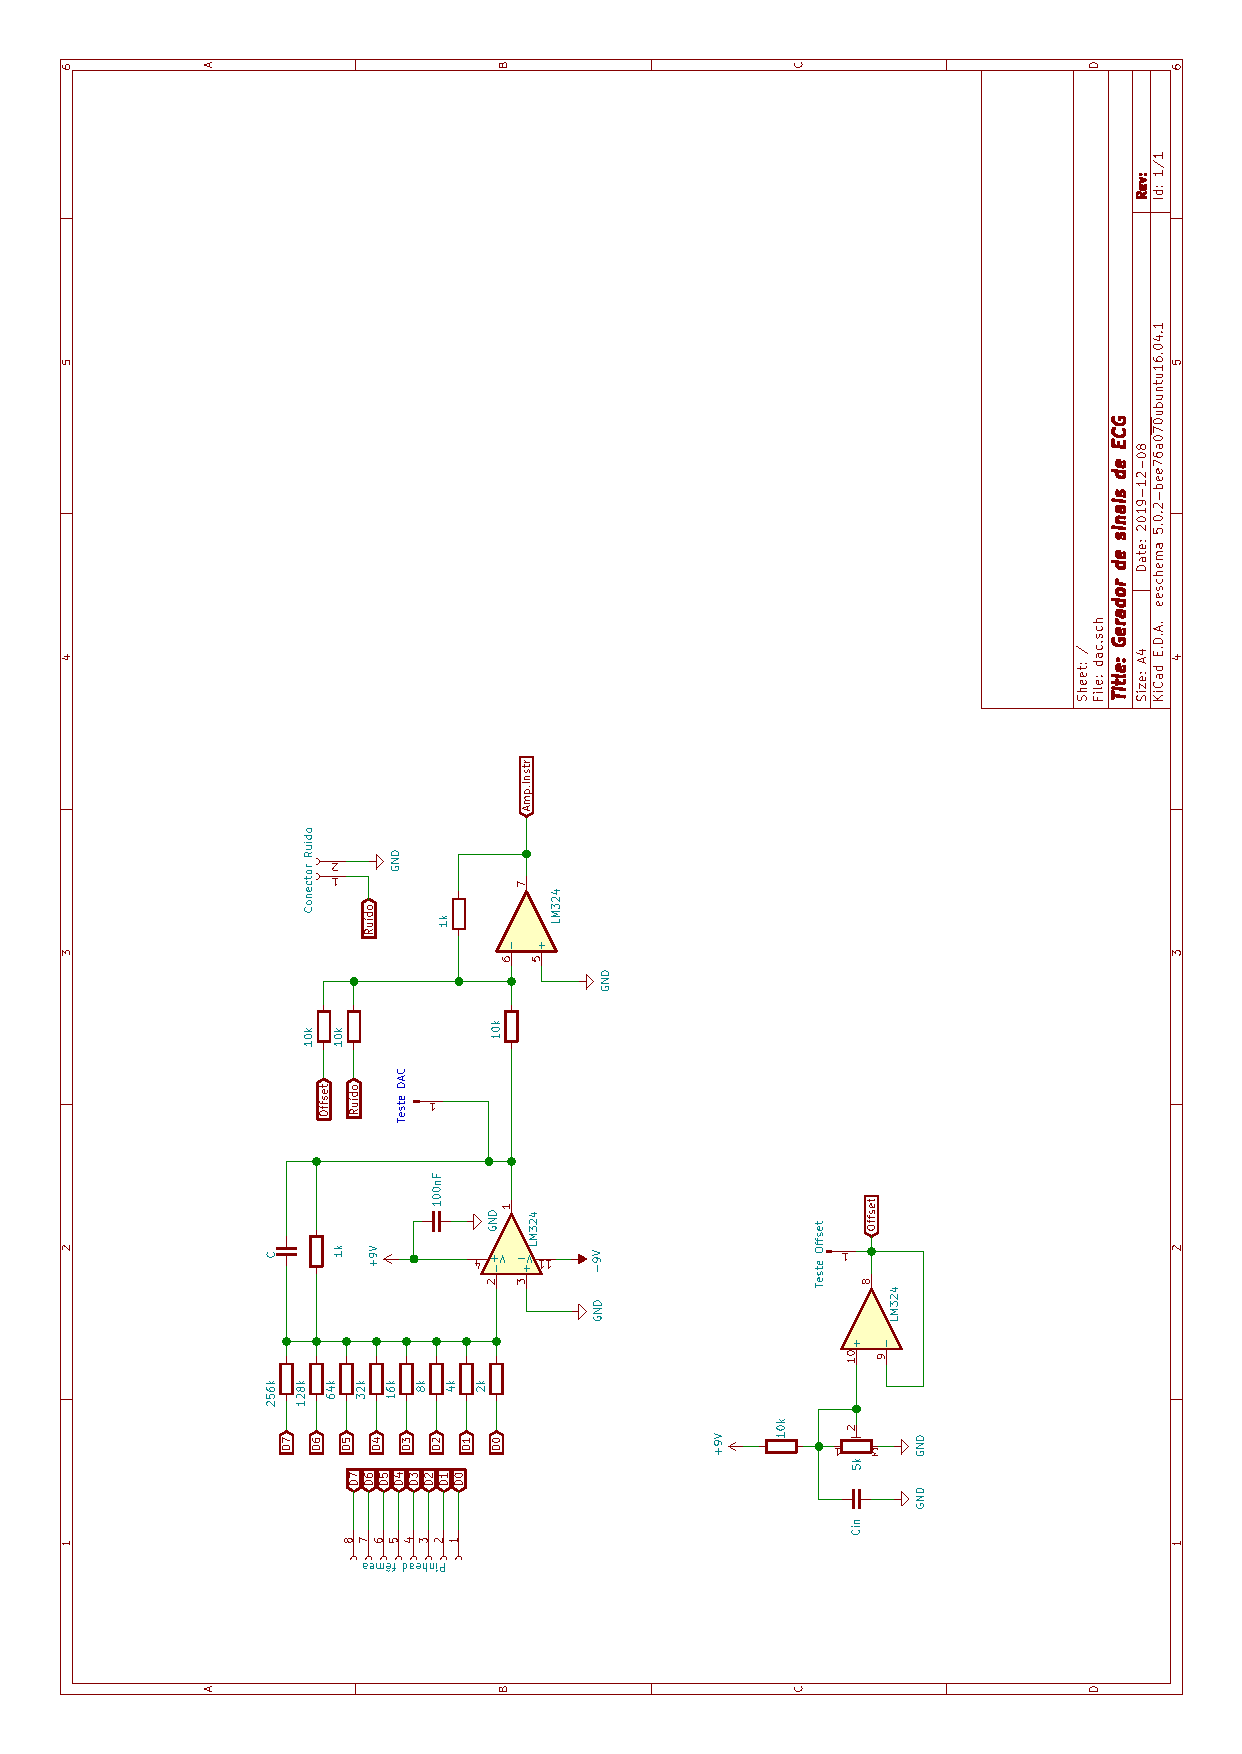
\includepdf[page={1}]{imagens/dac.pdf}

\end{document}
